\documentclass[10pt,xcolor=pst,aspectratio=169]{beamer}

\usepackage{etex}

%\usetheme{Boadilla}
%\usecolortheme{wolverine}
\usecolortheme{dolphin}
%\setbeamercovered{transparent}
%\setbeamercolor{block body}{bg=yellow}

\addtobeamertemplate{navigation symbols}{}{%
	\usebeamerfont{footline}%
	\usebeamercolor[fg]{footline}%
	\hspace{1em}%
	\insertframenumber/\inserttotalframenumber
}

\usepackage[utf8]{inputenc}
\usepackage[english,russian]{babel}
\usepackage[OT1]{fontenc}
\usepackage{amsmath, bm}
\usepackage{amsfonts}
\usepackage{amssymb}
\usepackage{graphicx}
\usepackage{wrapfig}
\usepackage[3D]{movie15}
\usepackage{animate}
\usepackage{ragged2e}
\usepackage{listings}
\usepackage{color}
\usepackage{pst-all}

\usepackage{tikz}
\usetikzlibrary{
	mindmap,
	arrows, % стрелки
	shapes.misc, % фигуры
	chains, % цепочки
	positioning, % позиционирование элементов
	scopes, % создание дополнительных веток
	shadows % тени
}

\graphicspath{{pic/}}

\author{\textbf{Губкин А.С.}}

\title[Решение СЛАУ]{Решение систем линейных алгебраических уравнений}

\logo{
\includegraphics[width=0.1\linewidth]{LOGO_2.PNG}}

\institute[ТюмФ ИТПМ СО РАН]{Тюменский филиал Института теоретической и прикладной механики\\ им. С. А. Христиановича СО РАН, г. Тюмень}

%\date{6 октября 2015 г.}

\begin{document}

\lstset{ %
	language=[ANSI]C++,                 % выбор языка для подсветки (здесь это С++)
	keywordstyle=\color{blue},
	commentstyle=\color{gray},
	basicstyle=\scriptsize,
	%basicstyle=\small\sffamily, % размер и начертание шрифта для подсветки кода
	numbers=left,               % где поставить нумерацию строк (слева\справа)
	numberstyle=\tiny,           % размер шрифта для номеров строк
	%stepnumber=1,                   % размер шага между двумя номерами строк
	numbersep=4pt,                % как далеко отстоят номера строк от подсвечиваемого кода
	%backgroundcolor=\color{white}, % цвет фона подсветки - используем \usepackage{color}
	showspaces=false,            % показывать или нет пробелы специальными отступами
	showstringspaces=false,      % показывать или нет пробелы в строках
	showtabs=false,             % показывать или нет табуляцию в строках
	frame=single,              % рисовать рамку вокруг кода
	%tabsize=2,                 % размер табуляции по умолчанию равен 2 пробелам
	captionpos=t,              % позиция заголовка вверху [t] или внизу [b] 
	breaklines=true,           % автоматически переносить строки (да\нет)
	breakatwhitespace=true, % переносить строки только если есть пробел
	escapeinside={\%*}{*)}   % если нужно добавить комментарии в коде
}

%SLIDE
\begin{frame}

	\transdissolve[duration=0.2]
	\titlepage

\end{frame}

%SLIDE
\begin{frame}{Введение}

	\transdissolve[duration=0.2]
	\justifying
	\large
	Задачи, приводящие к системам линейных алгебраических уравнений (СЛАУ): \pause
	\begin{itemize} \justifying
		\item статический анализ конструкций (мост, здание, несущая конструкция самолета); \pause
		\item проектирование электрических цепей; \pause
		\item \textbf{численное решение дифференциальных уравнений}.
	\end{itemize}

\end{frame}

%SLIDE
\begin{frame}{Система линейных алгебраических уравнений}

	\transdissolve[duration=0.2]
	\justifying
	\large
	\begin{equation}
		\textbf{A} \cdot \textbf{x} = \textbf{b}
		\label{eqn:SLAE_VEC}
	\end{equation}
	\begin{equation}
		\begin{cases}
			a_{1 1} x_{1} + a_{1 2} x_{2} + \ldots a_{1 n} x_{n} & = b_{1} \\
			\vdots \\
			a_{n 1} x_{1} + a_{n 2} x_{2} + \ldots a_{n n} x_{n} & = b_{n} \\
		\end{cases}
		\label{eqn:SLAE_SCAL}
	\end{equation}
	Существование и единственность решения этой системы гарантируется при $\det \, \textbf{A} \neq 0$.

\end{frame}

%SLIDE
\begin{frame}{Задачи вычислительной линейной алгебры}

	\transdissolve[duration=0.2]
	\justifying
	\large
	\pause
	\begin{itemize}
	\item Решение систем линейных алгебраических уравнений:
		\[
			\textbf{A} \cdot \textbf{x} = \textbf{b} .
		\] \pause
	\item Вычисление определителей и обратных матриц:
		\[
			\det \, \textbf{A}, \; \textbf{B} = \textbf{A}^{-1} .
		\] \pause
	\item Вычисление собственных чисел и векторов:
		\[
			\textbf{A} \cdot \textbf{z}_{n} = \lambda_{n} \textbf{z}_{n} .
		\]
	\end{itemize}

\end{frame}

%SLIDE
\begin{frame}{Прямые и итерационные методы решения СЛАУ}

	\transdissolve[duration=0.2]
	\justifying
	Методы решения СЛАУ иожно разделить на два класса: \pause
	\begin{itemize} \justifying
		\item \textbf{\textcolor{blue}{Прямые методы}}. Данные методы позволяют получить точное решение задачи (без учета ошибок округления) за конечное число арифметических действий. \pause
		\item \textbf{\textcolor{blue}{Итерационные методы}} или \textbf{\textcolor{blue}{методы последовательных приближений}}. Позволяют вычислять последовательность векторов $\textbf{x}_{k}$, которая при $k \rightarrow \infty$ сходится к решннию задачи. На практике используют некоторое конечное приближение в зависимости от допустимого уровня погрешности.
	\end{itemize}

\end{frame}

%SLIDE
\begin{frame}{Метод Крамера}

	\transdissolve[duration=0.2]
	\justifying
	Известен явный способ получения решения СЛАУ - это метод Крамера:
	\[
		x_{i} = \frac{\vartriangle_{i}}{\vartriangle},
	\]
	где $\vartriangle$ -- определитель матрицы $\textbf{A}$, а $\vartriangle_{i}$ -- определитель матрицы, полученной из $\textbf{A}$ заменой $i$-го столбца на вектор $\textbf{b}$.
	Однако, вычислять определитель по формуле:
	\[
		\vartriangle = \sum_{i_1, i_2, \ldots, i_n} (-1)^{P(i_1, i_2, \ldots, i_n)} a_{1 i_1} a_{2 i_2} \ldots a_{n i_n}
	\]
	оказывается весьма затратно. Сложность вычисления методом Крамера составляет составляет $\mathcal{O} (n^2 \cdot n!)$. Практически этот метод применим лишь при небольших размерностях системы $n \lesssim 10$.

\end{frame}

%SLIDE
\begin{frame}{Итерационные методы}

	\transdissolve[duration=0.2]
	\justifying
	Итерационные методы обычно основываются на следующей эквивалентной форме системы (\ref{eqn:SLAE_VEC}):
	\begin{equation}
		\textbf{x} = \textbf{B} \cdot \textbf{x} + \textbf{g},
		\label{eqn:SLAE_ITER}
	\end{equation}
	где $\textbf{B}$ называется итерационной матрицей.
	Итерационный процесс формулируется на основе эквивалентной формы (\ref{eqn:SLAE_ITER}) в следующем виде:
	\begin{itemize}
		\item зададим начальное приближение (вектор) $\textbf{x}_{0}$;
		\item для каждого значения $k$ будем вычислять последующие приближения как
		\begin{center}
			$\textbf{x}_{k+1} = \textbf{B} \cdot \textbf{x}_{k} + \textbf{g}$;
		\end{center}
		\item если $\frac{\parallel \textbf{x}_{k+1} - \textbf{x}_{k} \parallel}{\parallel \textbf{x}_{k+1} \parallel} \leq \varepsilon$ или $\frac{\parallel \textbf{r}_{k+1} \parallel}{\parallel \textbf{x}_{k+1} \parallel} \leq \varepsilon$, тогда итерационный процесс завершен и мы полагаем, что $\textbf{x}_{\ast} = \textbf{x}_{k+1}$.
	\end{itemize}

\end{frame}

%SLIDE
\begin{frame}{Классические итерационные методы и релаксация}

	\transdissolve[duration=0.2]
	\justifying
	\large
	\begin{block}{Определение}
		Невязкой системы (\ref{eqn:SLAE_VEC}), соответствующей вектору $\textbf{x}$, будем называть вектор $\textbf{r} = \textbf{b} - \textbf{A} \cdot \textbf{x}$.
	\end{block}
	Исторически первые итерационные методы основывались на циклическом покомпонентном изменении вектора решения, осуществляемом таким образом, чтобы обнулить соответствующий коэффициент вектора невязки и тем самым уменьшить его норму. Подобная методика уточнения решения получила название релаксации.

\end{frame}

%SLIDE
\begin{frame}{Методы Якоби и Гаусса-Зейделя}

	\transdissolve[duration=0.2]
	\justifying
	\large
	Представим матрицу $\textbf{A}$ системы (\ref{eqn:SLAE_VEC}) в виде разности трех матриц:
	\[
		\textbf{A} = \textbf{D} - \textbf{E} - \textbf{F}.
	\]
	%FIG. #1
	\begin{figure}[h]
		\center{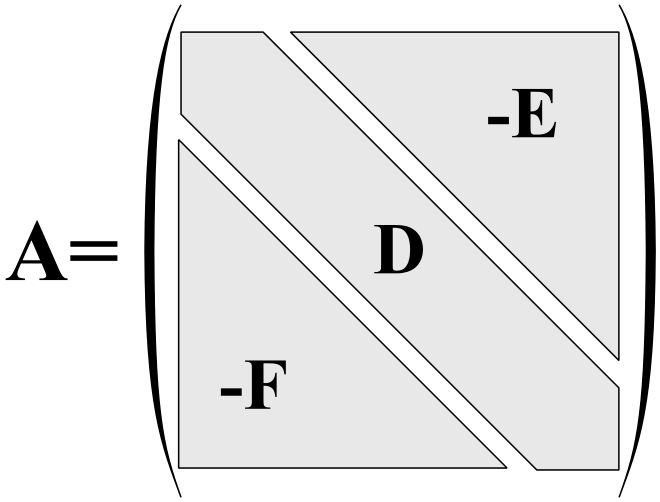
\includegraphics[width=0.5\linewidth]{A.png}}
	\end{figure}

\end{frame}

%SLIDE
\begin{frame}{Методы Якоби и Гаусса-Зейделя}

	\transdissolve[duration=0.2]
	\justifying
	\large
	Если имеется некоторое приближение $\textbf{x}_{k}$ к точному решению СЛАУ $\textbf{x}_{\ast}$, то при $\textbf{x}_{k} = \textbf{x}_{\ast}$ это соотношение не выполняется. Однако,
если в выражении
	\begin{equation}
		\textbf{A} \cdot \textbf{x}_{k} = \textbf{D} \cdot \textbf{x}_{k} - \textbf{E} \cdot \textbf{x}_{k} - \textbf{F} \cdot \textbf{x}_{k} = \textbf{b}
		\label{eqn:SIMPLE_ITER}
	\end{equation}
	одно или два из вхождений вектора $\textbf{x}_{k}$ заменить на $\textbf{x}_{k+1}$ и потребовать, чтобы равенство имело место, можно получить некоторую вычислительную схему для уточнения решения.

\end{frame}

%SLIDE
\begin{frame}{Метод Якоби (векторная форма)}

	\transdissolve[duration=0.2]
	\justifying
	\large
	Наиболее простой с точки зрения объема вычислительной работы вариант получается при замене в (\ref{eqn:SIMPLE_ITER}) $\textbf{D} \cdot \textbf{x}_{k}$ на $\textbf{D} \cdot \textbf{x}_{k+1}$. При этом получается схема:
	\begin{equation}
		\textbf{x}_{k+1} = \textbf{D}^{-1} \cdot (\textbf{E} + \textbf{F}) \cdot \textbf{x}_{k} + \textbf{D}^{-1} \cdot \textbf{b},
		\label{eqn:JACOBI_VEC}
	\end{equation}
	известная как метод Якоби.

\end{frame}

%SLIDE
\begin{frame}{Метод Якоби (скалярная форма)}

	\transdissolve[duration=0.2]
	\justifying
	\large
	Выражение (\ref{eqn:JACOBI_VEC}) в скалярной форме имеет вид:
	\begin{equation}
		x_{i}^{(k+1)} = \frac{1}{a_{ii}} \left( b_{i} - \sum_{j = 1}^{i - 1} a_{ij} x_{j}^{(k)} - \sum_{j = i + 1}^{n} a_{ij} x_{j}^{(k)} \right), \; i = 1,n.
		\label{eqn:JACOBI_SCAL}
	\end{equation}

\end{frame}

%SLIDE JACOBI_SRC
\begin{frame}[fragile]{Метод Якоби (исходный код)}

	\transdissolve[duration=0.2]
	\begin{lstlisting}
do{
    for(i = 0 ; i < N ; i++)
    {
        sum = 0.0;
        for(j = 0 ; j < N ; j++)
            sum = sum + matrix[i][j] * x_prev[j];
        x[i] = rhs[i] + sum;
    }
    sum = 0;
    sum_err = 0;
    for(i = 0 ; i < N ; i++)
    {
        sum = sum + x[i] * x[i];
        sum_err = sum_err + (x[i] - x_prev[i]) * (x[i] - x_prev[i]);
        x_prev[i] = x[i];
    }
    solution_log << "iteration #" << ++k << "\t eps = " << sqrt(sum_err / sum) << endl;
}while(sqrt(sum_err / sum) > eps);
	\end{lstlisting}

\end{frame}

%SLIDE
\begin{frame}{Метод Гаусса-Зейделя (скалярная форма)}

	\transdissolve[duration=0.2]
	\justifying
	\large
	Очевидным недостатком схемы (\ref{eqn:JACOBI_VEC}) -- (\ref{eqn:JACOBI_SCAL}) является то, что при нахождении $x_{i}^{(k+1)}$ никак не используется информация о уже пересчитанных компонентах $x_{1}^{(k+1)}, \ldots, x_{i-1}^{(k+1)}$. Исправить этот недостаток можно, переписав (\ref{eqn:JACOBI_SCAL}) в виде:
	\[
		x_{i}^{(k+1)} = \frac{1}{a_{ii}} \left( b_{i} - \sum_{j = 1}^{i - 1} a_{ij} x_{j}^{(k+1)} - \sum_{j = i + 1}^{n} a_{ij} x_{j}^{(k)} \right),  i = 1,n.
	\]

\end{frame}

%SLIDE GAUSS_SEIDEL_SRC
\begin{frame}[fragile]{Метод Гаусса-Зейделя (исходный код)}

	\transdissolve[duration=0.2]
	\begin{lstlisting}
do{
    for(i = 0 ; i < N ; i++)
    {
        sum = 0;
        x_prev[i] = x[i];
        for(j = 0 ; j < N ; j++)
            sum = sum + matrix[i][j]*x[j];
        x[i] = rhs[i] + sum;
    }
    sum = 0;
    sum_err = 0;
    for(i = 0 ; i < N ; i++)
    {
        sum = sum + x[i] * x[i];
        sum_err = sum_err + (x[i] - x_prev[i]) * (x[i] - x_prev[i]);
    }
    solution_log << "iteration #" << ++k << "\t eps = " << sqrt(sum_err / sum) << endl;
}while(sqrt(sum_err / sum) > eps);
	\end{lstlisting}

\end{frame}

%SLIDE
\begin{frame}{Метод Гаусса - Зейделя (векторная форма)}

	\transdissolve[duration=0.2]
	\justifying
	\large
	Векторную форму метода Гаусса-Зейделя можно получить из (\ref{eqn:SIMPLE_ITER}) заменой $\textbf{x}_{k}$ на $\textbf{x}_{k+1}$ при матрицах $\textbf{D}$ и $\textbf{E}$, т.е.:
	\[
		\textbf{x}_{k+1} = (\textbf{D} - \textbf{E})^{-1} \cdot \textbf{F} \cdot \textbf{x}_{k} + (\textbf{D} - \textbf{E})^{-1} \cdot \textbf{b}.
	\]
	Если вместо этой пары матриц взять $\textbf{D}$ и $\textbf{F}$, то получится похожая схема:
	\[
		\textbf{x}_{k+1} = (\textbf{D} - \textbf{F})^{-1} \cdot \textbf{E} \cdot \textbf{x}_{k} + (\textbf{D} - \textbf{F})^{-1} \cdot \textbf{b},
	\]
которая называется \textbf{\textcolor{blue}{обратным методом Гаусса - Зейделя}}

\end{frame}

%SLIDE REVERSE_GAUSS_SEIDEL_SRC
\begin{frame}[fragile]{Обратный метод Гаусса - Зейделя (исходный код)}

	\transdissolve[duration=0.2]
	\begin{lstlisting}
do{
    for(i = N - 1 ; i >= 0 ; i--)
    {
        sum = 0;
        x_prev[i] = x[i];
        for(j = 0 ; j < N ; j++)
            sum = sum + matrix[i][j]*x[j];
        x[i] = rhs[i] + sum;
    }
    sum = 0;
    sum_err = 0;
    for(i = 0 ; i < N ; i++)
    {
        sum = sum + x[i] * x[i];
        sum_err = sum_err + (x[i] - x_prev[i]) * (x[i] - x_prev[i]);
    }
    solution_log << "iteration #" << ++k << "\t eps = " << sqrt(sum_err / sum) << endl;
}while(sqrt(sum_err / sum) > eps);
	\end{lstlisting}

\end{frame}

%SLIDE
\begin{frame}{Симметричный
метод Гаусса-Зейделя}

	\transdissolve[duration=0.2]
	\justifying
	\large
	Еще одной модификацией является симметричный метод Гаусса-Зейделя, который заключается в циклическом чередовании \textbf{\textcolor{blue}{прямого}} и \textbf{\textcolor{blue}{обратного}} метода Гаусса - Зейделя на соседних итерациях:
	\[
		\begin{cases}
			\textbf{x}_{k+1} = (\textbf{D} - \textbf{E})^{-1} \cdot \textbf{F} \cdot \textbf{x}_{k} + (\textbf{D} - \textbf{E})^{-1} \cdot \textbf{b} \\
			\textbf{x}_{k+1} = (\textbf{D} - \textbf{F})^{-1} \cdot \textbf{E} \cdot \textbf{x}_{k} + (\textbf{D} - \textbf{F})^{-1} \cdot \textbf{b}
		\end{cases}
	\]

\end{frame}

%SLIDE
\begin{frame}{Расщепление}

	\transdissolve[duration=0.2]
	\justifying
	\large
	Все предыдущие методы можно записать в виде:
	\[
		\textbf{K} \cdot \textbf{x}_{k+1} = \textbf{R} \cdot \textbf{x}_{k} + \textbf{b},
	\]
	где матрицы $\textbf{K}$ и $\textbf{R}$ свзаны соотношением:
	\[
		\textbf{A} = \textbf{K} - \textbf{R}.
	\]
	Подобное представление матрицы $\textbf{A}$ называется \textbf{\textcolor{blue}{расщеплением}}, а методы такого вида -- \textbf{\textcolor{blue}{методами, основанными на расщеплении}}. Очевидно, матрица $\textbf{K}$ должна быть невырожденной и легко обратимой.

\end{frame}

%SLIDE
\begin{frame}{Нормы векторов и матриц}

	\transdissolve[duration=0.2]
	\justifying
	\large
	Для исследования сходимости численных методов решения задач линейной алгебры вводятся понятия нормы векторов и матриц.
	\begin{block}{Определение}
		\justifying
		Нормой вектора $\textbf{х}$ (обозначают $\Vert \textbf{x} \Vert$) называназывают неотрицательное число, вычисляемое с помощью компонент вектора и обладающее следующими свойствами:
		\begin{itemize}
			\item $\Vert \textbf{x} \Vert \geq 0, \; \Vert \textbf{x} \Vert = 0 \Leftrightarrow \textbf{x} = \textbf{0}$.
			\item $\Vert \alpha \textbf{x} \Vert = \vert \alpha \vert \Vert \textbf{x} \Vert , \; \forall \alpha$.
			\item $\Vert \textbf{x} + \textbf{y} \Vert \leq \Vert \textbf{x} \Vert + \Vert \textbf{y} \Vert$.
		\end{itemize}
	\end{block}

\end{frame}

%SLIDE
\begin{frame}{Нормы векторов и матриц}

	\transdissolve[duration=0.2]
	\justifying
	\large
	\begin{block}{Определение}
		\justifying
		Нормой матрицы $\textbf{A}_{n \times n}$ (обозначается $\Vert \textbf{A} \Vert$) с вещественными элементами называют неотрицательное число, вычисляемое с помощью элементов матрицы и обладающее следующими свойствами:
		\begin{itemize}
			\item $\Vert \textbf{A} \Vert \geq 0, \; \Vert \textbf{A} \Vert = 0 \Leftrightarrow \textbf{A} = \textbf{0}$.
			\item $\Vert \alpha \textbf{A} \Vert = \vert \alpha \vert \Vert \textbf{A} \Vert , \; \forall \alpha$.
			\item $\Vert \textbf{A} + \textbf{B} \Vert \leq \Vert \textbf{A} \Vert + \Vert \textbf{B} \Vert$.
			\item $\Vert \textbf{A} \cdot \textbf{B} \Vert \leq \Vert \textbf{A} \Vert \Vert \textbf{B} \Vert$.
		\end{itemize}
	\end{block}

\end{frame}

%SLIDE
\begin{frame}{Нормы векторов и матриц}

	\transdissolve[duration=0.2]
	\justifying
	Норма матриц должна быть согласована с нормой векторов. Это согласование осуществляется связью:
	\[
		\Vert \textbf{A} \cdot \textbf{x} \Vert \leq \Vert \textbf{A} \Vert \Vert \textbf{x} \Vert .
	\]
	Наиболее употребительными являются следующие нормы векторов:
	\[
		\begin{split}
			\Vert \textbf{x} \Vert_{1} &= \max_{i} \vert x_{i} \vert , \\
			\Vert \textbf{x} \Vert_{2} &= \sum_{i = 1}^{n} \vert x_{i} \vert , \\
			\Vert \textbf{x} \Vert_{3} &= \sqrt{\sum_{i = 1}^{n} x_{i}^{2}} = (\textbf{x} , \textbf{x}) .
		\end{split}
	\]

\end{frame}

%SLIDE
\begin{frame}{Нормы векторов и матриц}

	\transdissolve[duration=0.2]
	\justifying
	Нормы матриц, согласованные с нормами векторов, будут соотвественно:
	\[
		\begin{split}
			\Vert \textbf{A} \Vert_{1} &= \max_{i} \sum_{j = 1}^{n} \vert a_{ij} \vert , \\
			\Vert \textbf{A} \Vert_{1} &= \max_{j} \sum_{i = 1}^{n} \vert a_{ij} \vert , \\
			\Vert \textbf{A} \Vert_{3} &= \sqrt{\max_{i} \vert \lambda_{i} \vert_{\textbf{A}^{T} \cdot \textbf{A}}} .
		\end{split}
	\]
	Под знаком квадратного корня в норме матрицы $\Vert \textbf{A} \Vert_{3}$ находится спектральный радиус симметрической матрицы $\textbf{A}^{T} \cdot \textbf{A}$, для которой все собственные значения являются действительными.

\end{frame}

%SLIDE
\begin{frame}{Нормы векторов и матриц}

	\transdissolve[duration=0.2]
	\justifying
	\large
	Из линейной алгебры известно, что собственные значения матриц не превышают их норм. Действительно, из равенства $\textbf{А} \cdot \textbf{x} = \lambda \textbf{x}$ и свойств норм векторов и матриц следует: $\Vert \lambda \textbf{x} \Vert = \vert \lambda \vert \Vert \textbf{x} \Vert = \Vert \textbf{A} \cdot \textbf{x} \Vert \leq \Vert \textbf{A} \Vert \Vert \textbf{x} \Vert \Rightarrow \vert \lambda \vert \leq \Vert \textbf{A} \Vert$, или $\rho(\textbf{А}) \leq \Vert \textbf{A} \Vert$, где $\rho(\textbf{А}) = \max_{i} \vert \lambda_{i} \vert$ -- максимальное по модулю собственное значение или спектральный радиус матрицы $\textbf{A}$. Таким образом, за норму матрицы можно принять ее спектральный радиус.

\end{frame}

%SLIDE
\begin{frame}{Теорема о сходимости итерационного метода}

	\transdissolve[duration=0.2]
	\justifying
	\large
	Условия сходимости изложенных методов устанавливает следующая теорема:
	\begin{block}{Теорема}
		\justifying
		Вычислительная схема сходится при любом начальном приближении $\textbf{x}_{0}$ тогда и только тогда, когда матрицы $\textbf{K}$ и $\textbf{R}$ удовлетворяют условию
		\[
			\max_{j} \vert \lambda_{j} (\textbf{K}^{-1} \cdot \textbf{R}) \vert < 1.
		\]
	\end{block}

\end{frame}

%SLIDE
\begin{frame}{Теорема о сходимости итерационного метода}

	\transdissolve[duration=0.2]
	\justifying
	\begin{block}{Доказательство}
		\justifying
		Пусть известно точно решение СЛАУ $\textbf{x}_{\ast}$, тогда:
		\[
			\begin{cases}
				\textbf{K} \cdot \textbf{x}_{k+1} & = \textbf{R} \cdot \textbf{x}_{k} + \textbf{b} \\
				\textbf{K} \cdot \textbf{x}_{\ast} & = \textbf{R} \cdot \textbf{x}_{\ast} + \textbf{b}
			\end{cases} \Rightarrow \textbf{K} \cdot (\textbf{x}_{\ast} - \textbf{x}_{k+1}) = \textbf{R} \cdot (\textbf{x}_{\ast} - \textbf{x}_{k}) \Rightarrow
		\]
		\[
			\begin{split}
				& \textbf{K} \cdot \varepsilon_{k+1} = \textbf{R} \cdot \varepsilon_{k} \Rightarrow \varepsilon_{k+1} = \textbf{K}^{-1} \cdot \textbf{R} \cdot \varepsilon_{k} = (\textbf{K}^{-1} \cdot \textbf{R})^{k+1} \cdot \varepsilon_{0} \Rightarrow \\
				& \Vert \varepsilon_{k+1} \Vert = \Vert (\textbf{K}^{-1} \cdot \textbf{R})^{k+1} \Vert \cdot \Vert \varepsilon_{0} \Vert = \left(\sqrt{\max_{i} \vert \lambda_{i} (\textbf{K}^{-1} \cdot \textbf{R}) \vert} \right)^{k+1} \Vert \varepsilon_{0} \Vert
			\end{split}
		\]
		Следовательно, для сходимости необходимо и достаточно выполнения условия $\Vert \textbf{K}^{-1} \cdot \textbf{R} \Vert^{k} \rightarrow 0$ при $k \rightarrow \infty$.
	\end{block}

\end{frame}

%SLIDE
\begin{frame}{Ускорение сходимости релаксационных методов. Методы SOR и SSOR}

	\transdissolve[duration=0.2]
	\justifying
	\begin{block}{Следствие из теоремы}
		\justifying
		Чем меньше величина $\max_{j} \vert \lambda_{j} (\textbf{K}^{-1} \cdot \textbf{R}) \vert$, тем быстрее сходимость метода.
	\end{block}
	Одним из распространенных способов улучшения сходимости является введение параметра.
	\[
		\omega \textbf{A} \cdot \textbf{x} = \omega \textbf{b}.
	\]
	Представим матрицу $\omega \textbf{A}$ в виде:
	\[
		\omega \textbf{A} = (\textbf{D} - \omega \textbf{E}) - (\omega \textbf{F} + (1 - \omega) \textbf{D}),
	\]
	тогда можно построить итерационную схему, похожую на метод Гаусса-Зейделя,
	\[
		(\textbf{D} - \omega \textbf{E}) \cdot \textbf{x}_{k+1} = (\omega \textbf{F} + (1 - \omega) \textbf{D}) \cdot \textbf{x}_{k} + \omega \textbf{b}.
	\]

\end{frame}

%SLIDE
\begin{frame}{Метод SOR}

	\transdissolve[duration=0.2]
	\justifying
	\large
	Такая схема называется методом последовательной верхней релаксации (\textbf{\textcolor{blue}{Successive Over Relaxation}} или сокращенно \textbf{\textcolor{blue}{SOR}}). Для нее
	\[
		\textbf{K}_{\texttt{SOR}} (\omega) = \textbf{D} - \omega \textbf{E},
	\]
	\[
		\textbf{R}_{\texttt{SOR}} (\omega) = \omega \textbf{F} + (1 - \omega) \textbf{D}.
	\]
	На практике было замечено, что такая итерационная  схема сходится медленне при $\omega < 1$ (нижняя релаксация), чем при $\omega \geqslant 1$ (верхняя релаксация).

\end{frame}

%SLIDE
\begin{frame}{Метод SOR (скалярная форма)}

	\transdissolve[duration=0.2]
	\justifying
	\large
	В методе \textbf{SOR} решение удовлетворяет соотношению:
	\[
		x_{i}^{(k+1)} = \omega x_{i}^{GS} + (1 - \omega) x_{i}^{(k)}, \; i = 1,n,
	\]
	где $x_{i}^{GS}$ итерация метода Гаусса-Зейделя.

\end{frame}

%SLIDE SOR_SRC
\begin{frame}[fragile]{Метод SOR (исходный код)}

	\transdissolve[duration=0.2]
	\begin{lstlisting}
do{
    for(i = 0 ; i < N ; i++)
    {
        sum = 0;
        for(j = 0 ; j < N ; j++)
            sum = sum + matrix[i][j] * x[j];
        x[i] = omega * (rhs[i] + sum) + (1 - omega) * x_prev[i];
    }
    sum = 0;
    sum_err = 0;
    for(i = 0 ; i < N ; i++)
    {
        sum = sum + x[i] * x[i];
        sum_err = sum_err + (x[i] - x_prev[i]) * (x[i] - x_prev[i]);
        x_prev[i] = x[i];
    }
    solution_log << "iteration #" << ++k << "\t eps = " << sqrt(sum_err / sum) << endl;
}while(sqrt(sum_err / sum) > eps);
	\end{lstlisting}

\end{frame}

%SLIDE
\begin{frame}{Обратный метод SOR}

	\transdissolve[duration=0.2]
	\justifying
	\large
	Если в выражении
	\[
		\omega \textbf{A} = (\textbf{D} - \omega \textbf{E}) - (\omega \textbf{F} + (1 - \omega) \textbf{D})
	\]
	поменять местами матрицы $\textbf{E}$ и $\textbf{F}$, то такая перестановка дает \textbf{\textcolor{blue}{обратный метод последовательной верхней релаксации}}:
	\[
		(\textbf{D} - \omega \textbf{F}) \cdot \textbf{x}_{k+1} = (\omega \textbf{E} + (1 - \omega) \textbf{D}) \cdot \textbf{x}_{k} + \omega \textbf{b}.
	\]

\end{frame}

%SLIDE SOR_SRC
\begin{frame}[fragile]{Метод RSOR (исходный код)}

	\transdissolve[duration=0.2]
	\begin{lstlisting}
do{
    for(i = N - 1 ; i >= 0 ; i--)
    {
        sum = 0;
        for(j = 0 ; j < N ; j++)
            sum = sum + matrix[i][j] * x[j];
        x[i] = omega * (rhs[i] + sum) + (1 - omega) * x_prev[i];
    }
    sum = 0;
    sum_err = 0;
    for(i = 0 ; i < N ; i++)
    {
        sum = sum + x[i] * x[i];
        sum_err = sum_err + (x[i] - x_prev[i]) * (x[i] - x_prev[i]);
        x_prev[i] = x[i];
    }
    solution_log << "iteration #" << ++k << "\t eps = " << sqrt(sum_err / sum) << endl;
}while(sqrt(sum_err / sum) > eps);
	\end{lstlisting}

\end{frame}

%SLIDE
\begin{frame}{Метод SSOR}

	\transdissolve[duration=0.2]
	\justifying
	\large
	Последовательное применение прямого и обратного методов \textbf{SOR} дает симметричный метод последовательной верхней релаксации (\textbf{\textcolor{blue}{Symmetric Successive Over Relaxation}} или сокращенно \textbf{\textcolor{blue}{SSOR}}):
	\[
		\begin{cases}
			(\textbf{D} - \omega \textbf{E}) \cdot \textbf{x}_{k+1} = (\omega \textbf{F} + (1 - \omega) \textbf{D}) \cdot \textbf{x}_{k} + \omega \textbf{b} \\
			(\textbf{D} - \omega \textbf{F}) \cdot \textbf{x}_{k+1} = (\omega \textbf{E} + (1 - \omega) \textbf{D}) \cdot \textbf{x}_{k} + \omega \textbf{b}
		\end{cases}
	\]

\end{frame}

%SLIDE #1 EXAMPLE
\begin{frame}{Пример}

	\transdissolve[duration=0.2]
	\justifying
	\large
	Рассмотрим предыдущие итерационные методы на примере СЛАУ с матрицей:
	\begin{equation}
		\textbf{A} =
		\begin{pmatrix}
n & 1 & \cdots & 1 \\
1 & n & \cdots & 1 \\        
\vdots & \vdots & \ddots & \vdots \\
1 & 1 & \cdots & n
		\end{pmatrix},
		\label{eqn:example_A}
	\end{equation}
	и вектором свободных членов:
	\begin{equation}
		\textbf{f} =
		\begin{pmatrix}
2 n - 1 \\
2 n - 1 \\        
\vdots \\
2 n - 1
		\end{pmatrix}.
		\label{eqn:example_f}
	\end{equation}

\end{frame}

%SLIDE #2 EXAMPLE
\begin{frame}{Пример}

	\transdissolve[duration=0.2]
	\justifying
	\large
	Решение СЛАУ (\ref{eqn:SLAE_VEC}) с матрицей (\ref{eqn:example_A}) и с вектором свободных членов (\ref{eqn:example_f}) известно и равно:
	\begin{equation}
		\textbf{x} =
		\begin{pmatrix}
1 \\
1 \\        
\vdots \\
1
		\end{pmatrix}.
	\end{equation}
	Положим $n = 100, \omega = 0.9, \varepsilon = 1e-10$.

\end{frame}

%SLIDE #3 EXAMPLE
\begin{frame}{Пример}

	\transdissolve[duration=0.2]
	\begin{block}{Метод Якоби}
		iteration \#1	 eps = 2.26422 \\
		iteration \#2	 eps = 1.80543 \\
		iteration \#3	 eps = 2.27005 \\
		$\cdots$ \\
		iteration \#2580	 eps = 9.91072e-11
	\end{block}
	\begin{block}{Метод Гаусса-Зейделя}
		iteration \#1	 eps = 3.3409 \\
		iteration \#2	 eps = 3.57371 \\
		iteration \#3	 eps = 0.672445 \\
		$\cdots$ \\
		iteration \#18	 eps = 5.85572e-11
	\end{block}

\end{frame}

%SLIDE #4 EXAMPLE
\begin{frame}{Пример}

	\transdissolve[duration=0.2]
	\begin{block}{Метод SOR}
		iteration \#1	 eps = 3.87681 \\
		iteration \#2	 eps = 3.45209 \\
		iteration \#3	 eps = 0.280227 \\
		$\cdots$ \\
		iteration \#16	 eps = 5.07988e-11
	\end{block}
	\begin{block}{Метод RSOR}
		iteration \#1	 eps = 3.87681 \\
		iteration \#2	 eps = 3.45209 \\
		iteration \#3	 eps = 0.280227 \\
		$\cdots$ \\
		iteration \#16	 eps = 5.07989e-11
	\end{block}

\end{frame}

%SLIDE #
\begin{frame}{Предобусловливание (левое)}

	\transdissolve[duration=0.2]
	\justifying
	\large
	Пусть $\textbf{M}$ -- некоторая невырожденная матрица размерности $n$, тогда система

	\[
		\textbf{M}^{-1} \textbf{A} \cdot \textbf{x} = \textbf{M}^{-1} \cdot \textbf{b},
	\]

	имеет тоже самое точное решение $\textbf{x}_{*}$, но матрица $\textbf{M}^{-1} \textbf{A}$ будет иметь иные спектральные характеристики, что ведет к изменению скорости сходимости.

	\begin{block}{}
		\justifying
		Такой переход с целью улучшения характеристик матрицы называют \textbf{предобусловливанием (переобусловливанием)}. $\textbf{M}$ -- матрица предобусловливателя.
	\end{block}

\end{frame}

%SLIDE #
\begin{frame}{Требования}

	\transdissolve[duration=0.2]
	\justifying
	\large
	\begin{itemize}
		\item $\textbf{M}$ должна быть близка к матрице $\textbf{A}$;
		\item $\textbf{M}$ должна быть легко вычислимой;
		\item $\textbf{M}$ должна быть легко обратимой.
	\end{itemize}

	\begin{block}{}
		\justifying
		Такое предобусловливание называется \textbf{левым} поскольку мы умножаем матрицу СЛАУ на матрицу предобусловливателя слева.
	\end{block}

\end{frame}

%SLIDE #
\begin{frame}{Предобусловливание (правое)}

	\transdissolve[duration=0.2]
	\justifying
	\large
	Другой возможный подход основан на переходе от исходной системы к системе

	\[
		\textbf{A} \textbf{M}^{-1} \cdot \textbf{y} = \textbf{b},
	\]

	у которой точное решение $\textbf{y}_{*}$ связано с точным решением $\textbf{x}_{*}$ исходной СЛАУ соотношением

	\[
		\textbf{x}_{*} = \textbf{M}^{-1} \cdot \textbf{y}_{*},
	\]

	\begin{block}{}
		\justifying
		Такое предобусловливание называется \textbf{правым} поскольку мы умножаем матрицу СЛАУ на матрицу предобусловливателя справа.
	\end{block}

\end{frame}

%SLIDE #
\begin{frame}{Связь с предобусловливанием}

	\transdissolve[duration=0.2]
	\justifying
	\large
	Методы релаксации могут быть представлены в виде:

	\[
		\textbf{K} \cdot \textbf{x}_{k+1} = \textbf{R} \cdot \textbf{x}_{k} + \textbf{b} \: \mbox{или} \: \textbf{x}_{k+1} = \textbf{G} \cdot \textbf{x}_{k} + \textbf{f}
	\]

	это соотношение можно рассматривать как итерационную схему для СЛАУ

	\[
		\left( \textbf{I} - \textbf{G} \right) \cdot \textbf{x}= \textbf{f},
	\]

	в которой

	\[
		\begin{split}
			&\textbf{f} = \textbf{M}^{-1} \cdot \textbf{b}; \\
			&\textbf{G} = \textbf{K}^{-1} \textbf{R} = \textbf{K}^{-1} \left( \textbf{K} - \textbf{A} \right) = \textbf{I} - \textbf{K}^{-1} \textbf{A}.
		\end{split}
	\]

\end{frame}

%SLIDE #
\begin{frame}{Связь методов релаксации с предобусловливанием}

	\transdissolve[duration=0.2]
	\justifying
	\large
	Таким образом, данная система эквивалентна системе

	\[
		\textbf{K}^{-1} \textbf{A} \cdot \textbf{x} = \textbf{K}^{-1} \cdot \textbf{b},
	\]

	т.е. предобусловленной СЛАУ с матрицей предобусловливания $\textbf{K}$. 

\end{frame}

%SLIDE #
\begin{frame}{Матрицы предобусловливателя}

	\transdissolve[duration=0.2]
	\justifying
	\large
	Для уже изученных методов

	\[
		\begin{split}
			&\textbf{K}_{J} = \textbf{D}; \\
			&\textbf{K}_{GS} = \textbf{D} - \textbf{E}; \\
			&\textbf{K}_{SOR} = \frac{1}{\omega} \left( \textbf{D} - \omega \textbf{E} \right); \\
			&\textbf{K}_{SSOR} = \frac{1}{\omega (2 - \omega)} \left( \textbf{D} - \omega \textbf{E} \right) \textbf{D}^{-1} \left( \textbf{D} - \omega \textbf{F} \right).
		\end{split}
	\]

\end{frame}

%SLIDE
\begin{frame}{Проекционные методы. Подпространства Крылова}

	\transdissolve[duration=0.2]
	\large
	\begin{block}{Определение}
		\justifying
		\textbf{\textcolor{blue}{Проекционные методы решения СЛАУ}} -- класс итерационных методов, в которых решается задача проектирования неизвестного вектора на некоторое пространство оптимально относительно другого некоторого пространства.
	\end{block}

\end{frame}

%SLIDE
\begin{frame}{Условие Петрова-Галёркина}

	\transdissolve[duration=0.2]
	\justifying
	Рассмотрим СЛАУ $\textbf{A} \cdot \textbf{x} = \textbf{f}$, где $\textbf{A}$ -- квадратная матрица размерности $\textbf{n}$. Пусть $\mathcal{K}$ и $\mathcal{L}$ -- два $m$-мерных подпространства пространства $\mathcal{R}^n$. Необходимо найти такой вектор $\textbf{x} \in \mathcal{K}$ , чтобы $\textbf{r}_{x} = \textbf{f} - \textbf{A} \cdot \textbf{x} \perp \mathcal{L}$, т.е. выполнялось условие:
	\begin{block}{}
		\begin{equation}
			\forall \textbf{l} \in \mathcal{L}: (\textbf{A} \cdot \textbf{x} , \textbf{l}) = (\textbf{f} , \textbf{l}),
		\end{equation}
	\end{block}
	или
	\begin{block}{}
		\begin{equation}
			\forall \textbf{l} \in \mathcal{L}: (\textbf{r}_{\textbf{x}} , \textbf{l}) = 0,
		\end{equation}
	\end{block}
	называемое \textbf{\textcolor{blue}{условием Петрова-Галёркина}}.\\
	\begin{block}{}
		Такая задача называется задачей проектирования решения $\textbf{x}$ на подпространство $\mathcal{K}$ ортогонально к подпространству $\mathcal{L}$.
	\end{block}

\end{frame}

%SLIDE #31
\begin{frame}{Условие Петрова-Галёркина}

	\transdissolve[duration=0.2]
	\justifying
	\large
	Пусть для исходной системы (\ref{eqn:SLAE_VEC}) известно некоторое приближение $\textbf{x}_{0}$ к решению $\textbf{x}_{\ast}$. Требуется уточнить его поправкой $\delta \textbf{x} \in \mathcal{K}$ таким образом, чтобы $\textbf{f} - \textbf{A} \cdot (\textbf{x}_{0} + \delta \textbf{x}) \perp \mathcal{L}$. Условие Петрова - Галеркина в этом случае можно записать в виде
	\begin{block}{}
		\begin{equation}
			\forall \textbf{l} \in \mathcal{L}: (\textbf{r}_{\textbf{x} + \delta \textbf{x}} , \textbf{l}) = (\textbf{f} - \textbf{A} \cdot \textbf{x} - \textbf{A} \cdot \delta \textbf{x} , \textbf{l}) = (\textbf{r}_{0} - \textbf{A} \cdot \delta \textbf{x} , \textbf{l}) = 0.
			\label{eqn:Petrov_Galerkin_1}
		\end{equation}
	\end{block}

\end{frame}

%SLIDE #32
\begin{frame}{Общая постановка задачи}

	\transdissolve[duration=0.2]
	\justifying
	\large
	Пусть $\dim \mathcal{K} = \dim \mathcal{L} = m$. Введем в подпространствах $\mathcal{K}$ и $\mathcal{L}$ базисы $\textbf{V} = [\textbf{v}_1, \textbf{v}_2 , ..., \textbf{v}_m]$ и $\textbf{W } = [\textbf{w}_1, \textbf{w}_2, ..., \textbf{w}_m ]$ соответственно. Нетрудно видеть, что (\ref{eqn:Petrov_Galerkin_1}) выполняется тогда и только тогда, когда:
	\begin{equation}
		\forall \, j \, (1 \leq j \leq m) : (\textbf{r}_{0} - \textbf{A} \cdot \delta \textbf{x} , \textbf{w}_j) = 0.
		\label{eqn:Petrov_Galerkin_2}
	\end{equation}
	можно записать $\textbf{x}_{\ast} - \textbf{x}_{0} = \delta \textbf{x} = \textbf{V} \cdot \textbf{y}$ где $\textbf{y} \in \mathcal{R}^{m}$ -- вектор
коэффициентов. Тогда (\ref{eqn:Petrov_Galerkin_2}) может быть записано в виде:
	\[
		\textbf{W}^{T} \cdot (\textbf{r}_{0} - \textbf{A} \cdot \textbf{V} \cdot \textbf{y}) = 0,
	\]
	откуда
	\[
		\textbf{y} = \left( \textbf{W}^{T} \cdot \textbf{A} \cdot \textbf{V} \right)^{-1} \cdot \textbf{W}^{T} \cdot \textbf{r}_{0}.
	\]

\end{frame}

%SLIDE #33
\begin{frame}{Общая постановка задачи}

	\transdissolve[duration=0.2]
	\justifying
	\large
	Таким образом, решение должно уточняться в соответствии с формулой:
	\[
		\textbf{x}_{1} = \textbf{x}_{0} + \textbf{V} \cdot \textbf{y} = \textbf{V} \cdot \left( \textbf{W}^{T} \cdot \textbf{A} \cdot \textbf{V} \right)^{-1} \cdot \textbf{W}^{T} \cdot \textbf{r}_{0}.
	\]
	из которой сразу вытекает важное требование: в практических реализациях проекционных методов подпространства $\mathcal{K}$ и $\mathcal{L}$ и их базисы должны выбираться так, чтобы матрица $\left( \textbf{W}^{T} \cdot \textbf{A} \cdot \textbf{V} \right)$ либо была малой размерности, либо имела простую структуру, удобную для обращения.

\end{frame}

%SLIDE #34
\begin{frame}{Алгоритм проекционного метода}

	\transdissolve[duration=0.2]
	\justifying
	\large
	\begin{block}{Алгоритм}
		В общем виде алгоритм любого метода проекционного класса может быть записан следующим образом:
		\begin{itemize}
			\item Выбираем пару подпространств $\mathcal{K}$ и $\mathcal{L}$.
			\item Построение для $\mathcal{K}$ и $\mathcal{L}$ базисов $\textbf{V} = [\textbf{v}_1, \textbf{v}_2 , ..., \textbf{v}_m]$ и $\textbf{W } = [\textbf{w}_1, \textbf{w}_2, ..., \textbf{w}_m ]$.
			\item $\textbf{r}_{0} = \textbf{f} - \textbf{A} \cdot \textbf{x}_{0}$.
			\item $\textbf{y} = \left( \textbf{W}^{T} \cdot \textbf{A} \cdot \textbf{V} \right)^{-1} \cdot \textbf{W}^{T} \cdot \textbf{r}_{0}$.
			\item $\textbf{x}_{1} = \textbf{x}_{0} + \textbf{V} \cdot \textbf{y}$.
		\end{itemize}
	\end{block}

\end{frame}

%SLIDE #35
\begin{frame}{Случай одномерных подпространств $\mathcal{K}$ и $\mathcal{L}$}

	\transdissolve[duration=0.2]
	\justifying
	\large
	Наиболее простой ситуацией является случай, когда пространства $\mathcal{K}$ и $\mathcal{L}$ одномерны. В этом случае их матричные базисы являются векторами: $\textbf{V} = [\textbf{v}]$ и $\textbf{W} = [\textbf{w}]$ и выражение $\textbf{x}_{1} = \textbf{x}_{0} + \textbf{V} \cdot \textbf{y}$, можно переписать как:
	\begin{equation}
		\textbf{x}_{k+1} = \textbf{x}_{k} + \gamma_{k} \textbf{v}_{k},
		\label{eqn:1D_ITER}
	\end{equation}
	где $\gamma_{k}$ -- неизвестный коэффициент, который легко находится из условия ортогональности $\textbf{r}_{k} - \textbf{A} (\gamma_{k} \textbf{v}_{k}) \perp \textbf{w}_{k}$:
	\[
		(\textbf{r}_{k} - \gamma_{k} \textbf{A} \cdot \textbf{v}_{k} , \textbf{w}_{k}) = (\textbf{r}_{k} , \textbf{w}_{k}) - \gamma_{k} (\textbf{A} \cdot \textbf{v}_{k} , \textbf{w}_{k}) = 0,
	\]
	откуда
	\[
		\gamma_{k} = \frac{(\textbf{r}_{k} , \textbf{w}_{k})}{(\textbf{A} \cdot \textbf{v}_{k} , \textbf{w}_{k})}.
	\]

\end{frame}

%SLIDE #36
\begin{frame}{Метод наискорейшего спуска}

	\transdissolve[duration=0.2]
	\justifying
	\large
	Выберем $\textbf{v}_{k} = \textbf{w}_{k} = \textbf{r}_{k}$. Тогда (\ref{eqn:1D_ITER}) примет вид:
	\[
		\textbf{x}_{k+1} = \textbf{x}_{k} + \frac{(\textbf{r}_{k} , \textbf{r}_{k})}{(\textbf{A} \cdot \textbf{r}_{k} , \textbf{r}_{k})} \textbf{r}_{k}.
	\]
	Данный метод есть \textbf{\textcolor{blue}{метод наискорейшего спуска}} (\textbf{\textcolor{blue}{Steepest Descent Method}} или сокращенно \textbf{\textcolor{blue}{SDM}}).\pause
	\begin{block}{Замечание}
		\justifying
		\textbf{\textcolor{red}{В практических задачах метод наискорейшего спуска обладает достаточно медленной сходимостью!}}
	\end{block}

\end{frame}

%SLIDE #37
\begin{frame}{Метод наискорейшего уменьшения невязки}

	\transdissolve[duration=0.2]
	\justifying
	\large
	Выберем $\textbf{v}_{k} = \textbf{A}^{T} \cdot \textbf{r}_{k}$ и $\textbf{w}_{k} = \textbf{A} \cdot \textbf{v}_{k}$. Тогда (\ref{eqn:1D_ITER}) примет вид:
	\[
		\textbf{x}_{k+1} = \textbf{x}_{k} + \frac{(\textbf{r}_{k} , \textbf{A} \cdot \textbf{A}^{T} \cdot \textbf{r}_{k})}{(\textbf{A} \cdot \textbf{A}^{T} \cdot \textbf{r}_{k} , \textbf{A} \cdot \textbf{A}^{T} \cdot \textbf{r}_{k})} \textbf{A}^{T} \cdot \textbf{r}_{k}.
	\]
	Данный метод есть \textbf{\textcolor{blue}{метод наискорейшего уменьшения невязки}} (\textbf{\textcolor{blue}{Residual norm Steepest Descent}} или сокращенно \textbf{\textcolor{blue}{RnSD}}).

\end{frame}

%SLIDE #38
\begin{frame}{Подпространства Крылова}

	\transdissolve[duration=0.2]
	\justifying
	При построении и реализации проекционных методов важную роль играют так называемые подпространства Крылова, часто выбираемые в качестве $\mathcal{K}$.
	\begin{block}{Определение}
		\justifying
		Подпространством Крылова размерности $m$, порожденным вектором $\textbf{v}$ и матрицей $\textbf{A}$ называется линейное пространство
		\[
			\mathcal{K}_{m} (\textbf{v} , \textbf{A}) = span \left\lbrace \textbf{v} , \textbf{A} \cdot \textbf{v} , \textbf{A}^{2} \cdot \textbf{v} , \ldots , \textbf{A}^{m - 1} \cdot \textbf{v} \right\rbrace .
		\]
	\end{block}
	В качестве вектора $\textbf{v}$ обычно выбирается невязка начального приближения $\textbf{r}_{0}$; тогда выбор подпространства $\mathcal{L}$ и способ построения базисов подпространств полностью определяет вычислительную схему метода.

\end{frame}

%SLIDE #39
\begin{frame}{Подпространства Крылова?}

	\transdissolve[duration=0.2]
	\justifying
	\large
	Было показано, что методы Якоби и Гаусса - Зейделя являются частными случаями класса методов, основанного на расщеплении $\textbf{A}$ в виде разности $\textbf{A} = \textbf{K} - \textbf{R}$. Тогда исходная система (\ref{eqn:SLAE_VEC}) может быть записана в виде:
	\[
		\textbf{K} \cdot \textbf{x} = \textbf{f} + \textbf{R} \cdot \textbf{x} = \textbf{f} + (\textbf{K} - \textbf{A}) \cdot \textbf{x} ,
	\]
	что позволяет построить итерационный процесс:
	\[
		\textbf{K} \cdot \textbf{x}_{k+1} = \textbf{K} \cdot \textbf{x}_{k} + (\textbf{f} - \textbf{A} \cdot \textbf{x}_{k}) \Rightarrow \textbf{x}_{k+1} = \textbf{x}_{k} + \textbf{K}^{-1} \cdot \textbf{r}_{k}.
	\]

\end{frame}

%SLIDE #40
\begin{frame}{Подпространства Крылова?}

	\transdissolve[duration=0.2]
	\justifying
	\large
	Выберем $\textbf{K} = \textbf{I}$ и $\textbf{R} = \textbf{I} - \textbf{A}$, тогда предыдущий итерационный процесс будет сведен к виду:
	\[
		\textbf{x}_{k+1} = \textbf{x}_{k} + \textbf{r}_{k} \Rightarrow \textbf{x}_{k} = \textbf{x}_{0} + \textbf{r}_{0} + \textbf{r}_{1} + \ldots + \textbf{r}_{k - 1}.
	\]
	Умножив обе части слева на $- \textbf{A}$ и прибавив к ним $\textbf{f}$, получим
	\[
		\textbf{r}_{k + 1} = \textbf{f} - \textbf{A} \cdot \textbf{x}_{k+1} = \textbf{f} - \textbf{A} \cdot \textbf{x}_{k} - \textbf{A} \cdot \textbf{r}_{k} = \textbf{r}_{k} - \textbf{A} \cdot \textbf{r}_{k}.
	\]
	что позволяет найти выражение для невязки на $k$-ой итерации через невязку начального приближения:
	\[
		\textbf{r}_{k} = (\textbf{I} - \textbf{A}) \cdot \textbf{r}_{k - 1} = (\textbf{I} - \textbf{A})^{k} \cdot \textbf{r}_{0}.
	\]

\end{frame}

%SLIDE #41
\begin{frame}{Подпространства Крылова?}

	\transdissolve[duration=0.2]
	\justifying
	\large
	Таким образом:
	\[
		\textbf{x}_{k} = \textbf{x}_{0} + \left[ \sum_{j = 0}^{k - 1} (\textbf{I} - \textbf{A})^{j} \right] \cdot \textbf{r}_{0} ,
	\]
	т.е. $\delta\textbf{x} \in span \left\lbrace \textbf{r}_{0} , \textbf{A} \cdot \textbf{r}_{0} , \textbf{A}^{2} \cdot \textbf{r}_{0} , \ldots , \textbf{A}^{k - 1} \cdot \textbf{r}_{0} \right\rbrace = \mathcal{K}_{k}(\textbf{r}_{0} , \textbf{A}) .$
	\pause
	\begin{block}{Следствие}
		\justifying
		В методах, использующих подпространства Крылова, невязка на $k$-ой итерации выражается через начальную невязку некоторым матричным полиномом.
	\end{block}

\end{frame}

%SLIDE #42
\begin{frame}{Ортогонализация}

	\transdissolve[duration=0.2]
	\justifying
	\large
	\begin{block}{Ортогонализация}
		\justifying
		Это алгоритм, в которых на основе счётного множества линейно независимых векторов $\mathbf{a}_1,\;\ldots,\;\mathbf{a}_N$ строится множество ортогональных векторов $\mathbf{b}_1,\;\ldots,\;\mathbf{b}_N$ или ортонормированных векторов $\mathbf{e}_1,\;\ldots,\;\mathbf{e}_N$, причём так, что каждый вектор $\mathbf{b}_j$ или $\mathbf{e}_j$ может быть выражен линейной комбинацией векторов $\mathbf{a}_1,\;\ldots,\;\mathbf{a}_j$.
	\end{block}

\end{frame}

%SLIDE #43
\begin{frame}{Оператор проекции}

	\transdissolve[duration=0.2]
	\justifying
	\large
	Пусть имеются линейно независимые векторы $\mathbf{a}_1,\;\ldots,\;\mathbf{a}_N$.\\
	Определим оператор проекции следующим образом:\\
    \[
		\mathbf{proj}_{\mathbf{b}}\,\mathbf{a} = {\langle \mathbf{a}, \mathbf{b} \rangle \over \langle \mathbf{b}, \mathbf{b}\rangle} \mathbf{b} ,
	\]
	где $\langle \mathbf{a}, \mathbf{b} \rangle$ -- скалярное произведение векторов $\mathbf{a}$ и $\mathbf{b}$. Этот оператор проецирует вектор $\mathbf{a}$ коллинеарно вектору $\mathbf{b}$.

\end{frame}

%SLIDE #44
\begin{frame}{Ортогонализация Грама - Шмидта}

	\transdissolve[duration=0.2]
	\justifying
	\large
	Классический процесс Грама - Шмидта выполняется следующим образом:
	\[
		\begin{array}{lclr}
			\mathbf{b}_1 & = & \mathbf{a}_1 & \\
			\mathbf{b}_2 & = & \mathbf{a}_2-\mathbf{proj}_{\mathbf{b}_1}\,\mathbf{a}_2 & \\
			\mathbf{b}_3 & = & \mathbf{a}_3-\mathbf{proj}_{\mathbf{b}_1}\,\mathbf{a}_3-\mathbf{proj}_{\mathbf{b}_2}\,\mathbf{a}_3 & \\
			\mathbf{b}_4 & = & \mathbf{a}_4-\mathbf{proj}_{\mathbf{b}_1}\,\mathbf{a}_4-\mathbf{proj}_{\mathbf{b}_2}\,\mathbf{a}_4-\mathbf{proj}_{\mathbf{b}_3}\,\mathbf{a}_4 & \\
			& \vdots & & \\
			\mathbf{b}_N & = & \mathbf{a}_N-\displaystyle\sum_{j=1}^{N-1}\mathbf{proj}_{\mathbf{b}_j}\,\mathbf{a}_N & \end{array}
    \]

\end{frame}

%SLIDE #45
\begin{frame}{Нормированный базис}

	\transdissolve[duration=0.2]
	\justifying
	\large
	\[
		\mathbf{b}_j \Rightarrow \mathbf{e}_j = {\mathbf{b}_j \over \| \mathbf{b}_j \|}
	\]
	Результаты процесса Грама - Шмидта:
	\begin{itemize}
		\justifying
		\item $\mathbf{b}_1,\;\ldots,\;\mathbf{b}_N$ -- система ортогональных векторов либо
		\item $\mathbf{e}_1,\;\ldots,\;\mathbf{e}_N$ -- система ортонормированных векторов.
	\end{itemize}
	\begin{block}{}
		\justifying
		Вычисление $\mathbf{b}_1,\;\ldots,\;\mathbf{b}_N$ носит название \textbf{\textcolor{blue}{ортогонализации Грама - Шмидта}}, а $\mathbf{e}_1,\;\ldots,\;\mathbf{e}_N$ -- \textbf{\textcolor{blue}{ортонормализации Грама - Шмидта}}.
	\end{block}

\end{frame}

%SLIDE #46
\begin{frame}{Геометрическая интерпретация}

	\transdissolve[duration=0.2]
	\justifying
	\large
	\begin{center}
		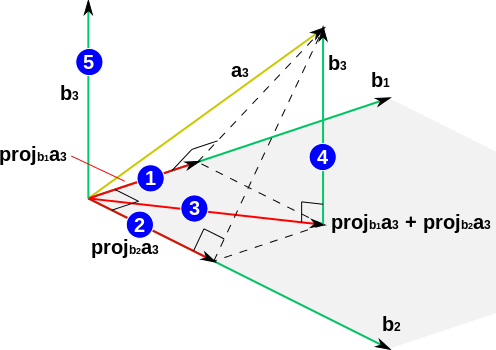
\includegraphics[width=0.8\linewidth]{Gram-schmidt-step3base.png}
	\end{center}

\end{frame}

%SLIDE #47
\begin{frame}{Базис подпространства Крылова. Ортогонализация Арнольди}

	\transdissolve[duration=0.2]
	\justifying
	\large
	Для построения базиса в пространстве Крылова $\mathcal{K}_{m} (\textbf{v}_{1} , \textbf{A})$ можно применить следующий подход. %Найдем сначала векторы w 1 = v 1 , w 2 = Aw 1 , w 3 = A 2 w 1 =
%= Aw 2 ,. . . , w m = A m?1 w 1 = Aw m?1 . По определению (4.10),
%K m (v 1 , A) = span{w 1 , w 2 , . . . , w m }.
%Перейдем теперь от {w 1 , w 2 , . . . , w m } к {v 1 , v 2 , . . . , v m }, применив
%процедуру ортогонализации
%k
%v k+1 = w k+1 ?
%? i v i
%i=1
%и затем пронормировав полученные векторы.

\end{frame}

\end{document}